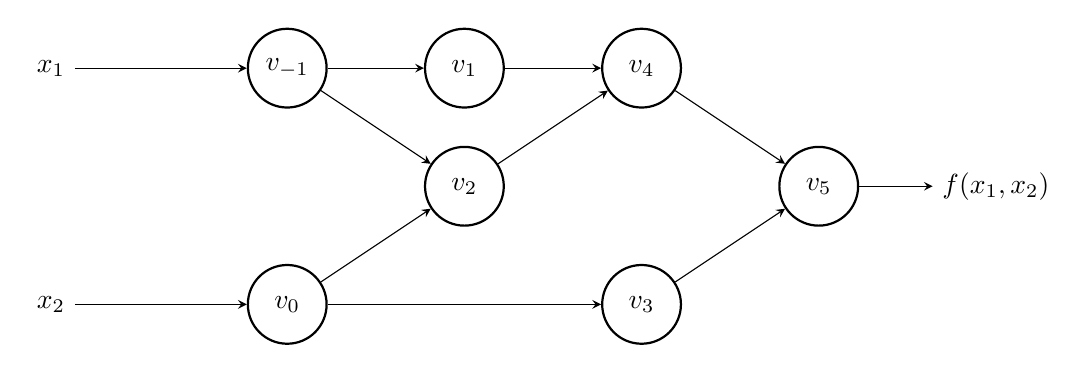
\begin{tikzpicture}[x=1.5cm, y=1.0cm, >=stealth]
\begin{scope}[]
    \node (x1) at (-2,1.5) {$x_1$};
    \node (x2) at (-2,-1.5) {$x_2$};
    \node (f) at (6,0) {$f(x_1, x_2)$} ;
\end{scope}

\begin{scope}[every node/.style={circle,thick,draw, minimum size=1cm}]
    \node (v-1) at (0,1.5)  {$v_{-1}$};
    \node (v1)  at (1.5,1.5)  {$v_1$};
    \node (v4)  at (3,1.5) {$v_4$};
    \node (v2)  at (1.5,0) {$v_2$};
    \node (v5)  at (4.5,0) {$v_5$};
    \node (v0)  at (0,-1.5) {$v_0$};
    \node (v3)  at (3,-1.5) {$v_3$};
\end{scope}

\begin{scope}[ ]
    \path [->] (x1) edge (v-1);
    \path [->] (v-1) edge (v1);
    \path [->] (v-1) edge (v2);
    \path [->] (v1) edge (v4);
    \path [->] (v2) edge (v4);
    \path [->] (v4) edge (v5);
    \path [->] (x2) edge (v0);
    \path [->] (v0) edge (v3);
    \path [->] (v0) edge (v2);
    \path [->] (v3) edge (v5);
    \path [->] (v5) edge (f);
\end{scope}
\end{tikzpicture}
